%%%%%%%%%%%%%%%%%%%%%%%%%%%%%%%%%%%%%%%%%%%%%%%%%%%%%%%%%%%%%%%%%%%%%%
% NeurIPS 2026 submission - Main Track (double-blind, anonymous).
% Derived from the tau-class progress report "Weight space regression
% for efficient continual learning" (see main_original_tau.tex for the
% un-trimmed source material).
%%%%%%%%%%%%%%%%%%%%%%%%%%%%%%%%%%%%%%%%%%%%%%%%%%%%%%%%%%%%%%%%%%%%%%

\documentclass{article}

% Main Track, preprint (non-anonymous for drafting; switch to anonymous for submission).
\usepackage[preprint]{neurips_2026}

\usepackage[utf8]{inputenc}
\usepackage[T1]{fontenc}
\usepackage[english]{babel}
\usepackage{hyperref}
\usepackage{url}
\usepackage{booktabs}
\usepackage{amsfonts}
\usepackage{amsmath,amssymb,amsthm,mathtools}
\usepackage{bbm}
\usepackage{nicefrac}
\usepackage{microtype}
\usepackage{xcolor}
\usepackage{graphicx}
\usepackage{array}
\usepackage{makecell}
\usepackage{ragged2e}
\usepackage[ruled,vlined,linesnumbered]{algorithm2e}
\usepackage{enumitem}

% --- lightweight notation macros (kept minimal to respect neurips style) ---
\newcommand{\wt}[1]{\tilde{w}_{#1}}       % ground-truth weights
\newcommand{\wh}[1]{\bar{w}_{#1}}          % predicted weights
\newcommand{\whft}[1]{\bar{\bar{w}}_{#1}}  % finetuned predicted weights
\newcommand{\PH}{\mathrm{PH}}
\newcommand{\SWD}{\mathrm{SWD}}
\newcommand{\Dg}{\operatorname{Dg}}

\title{Topological and Spectral Regularization for \\
       Weight-Space Regression in Class-Incremental Continual Learning}

\author{%
  Aymen Tlili \and Bassem Ben Hamed \\
  University of Sfax \\
  Sfax, Tunisia \\
  \texttt{aymen.tlili@enis.tn, bassem.benhamed@enis.tn}
}

\begin{document}

\maketitle

\begin{abstract}
Hyper-representation models compress a population of trained neural networks
into a latent space from which new, task-conditioned weights can be sampled.
Existing approaches rely on $\ell_2$ reconstruction of flattened parameter
vectors and produce networks that underperform until extensively
fine-tuned.  We argue that two intrinsic properties of the weight
distribution are systematically ignored by such objectives: the
\emph{topology} of the layer-wise point clouds (captured by persistent
homology and its multiparameter refinements) and the \emph{spectrum} of the
associated covariance operators (captured by Marchenko--Pastur statistics).
We instantiate this observation in a double-encoder Transformer that merges
the weights of two class-specialist CNNs into a third CNN handling the
union of classes, and regularize training with a differentiable composite
of (i)~layer-wise normalized MSE, (ii)~Sliced-Wasserstein distance between
persistence diagrams, and (iii)~a Fisher-weighted importance penalty.
Building on the algebraic-persistence framework of
\citet{oudotAlgebraicIntroductionPersistence2026} and the
multiparameter tooling of \citet{loiseauxStableVectorizationMultiparameter2024a,scoccolaDifferentiabilityOptimizationMultiparameter2024},
we show that the resulting latent space aligns predicted and ground-truth
weights in both their bar\-code structure and their eigenvalue bulk,
yielding a class-incremental CNN zoo that is merge-ready without extensive
fine-tuning.
\end{abstract}


\section{Introduction}
\label{sec:intro}

Continual learning aims to update a model on a stream of tasks without
catastrophic forgetting and without retraining from scratch
\citep{wangComprehensiveSurveyContinual2024,janv.2022ContinualLearningCourse}.
A recent line of work treats \emph{the trained weights themselves} as data:
a population of networks is collected into a \emph{model zoo} and a
meta-model (typically an auto-encoder or a diffusion model) learns to
generate task-conditioned parameters
\citep{schurholtHyperRepresentationsLearningPopulations2024,schurholtSelfSupervisedRepresentationLearning2021,schurholtHyperRepresentationsPreTrainingTransfer2022,soroDiffusionBasedNeuralNetwork2024,knyazevAcceleratingTrainingNeuron2025}.
If the generated weights already lie on, or very close to, the manifold
of high-performing parameters, downstream fine-tuning becomes cheap and
the hyper-representation doubles as a mechanism for knowledge merging,
unlearning and federated aggregation.

Existing hyper-representations are trained with Layer-Wise-Normalized MSE
and a contrastive auxiliary term
\citep{schurholtSelfSupervisedRepresentationLearning2021}.  We observe that
the MSE component is a very loose surrogate for functional similarity:
during fine-tuning, the $\ell_2$ error \emph{increases} while the
Wasserstein distance between weight distributions consistently decreases,
and classification accuracy improves.  This suggests that the geometry
exploited by fine-tuning is not point-wise but distributional and
topological.

\paragraph{Contributions.}
\begin{enumerate}[leftmargin=*,topsep=2pt,itemsep=1pt]
  \item We introduce a class-incremental MNIST weight zoo in which every
  sub-combination of digits is trained to convergence (not only to a weak
  $5$--$10$ epoch checkpoint as in prior zoos), together with a
  pair-merging benchmark exposing the effect of class overlap.
  \item We describe a double-encoder Transformer that fuses two class-specialist
  CNNs into a third CNN via a shared bottleneck and a sequence-of-tokens
  decoder.
  \item We formulate a \emph{differentiable} topological--spectral
  regularizer combining Sliced-Wasserstein distance between persistence
  diagrams (one-parameter and, optionally, multi-parameter in the sense
  of \citet{scoccolaDifferentiabilityOptimizationMultiparameter2024}) with
  a Marchenko--Pastur-based spectral penalty.
  \item We provide an empirical protocol reporting, for each
  (overlap, loss) configuration, persistent-homology statistics, Mapper
  graphs and eigenvalue distributions (Tables~\ref{tab:topo-metrics}--\ref{tab:layer-mean-std},
  Figures~\ref{fig:stat-patterns}--\ref{fig:eig-distribution}).
\end{enumerate}


\section{Related Work}
\label{sec:related}

\paragraph{Hyper-representations and weight generation.}
\citet{schurholtSelfSupervisedRepresentationLearning2021} introduced
auto-encoders over flattened weight vectors and showed that a single latent
space captures a meaningful distribution of trained CNNs.  Downstream work
scales this idea to larger zoos and diffusion-based samplers
\citep{schurholtHyperRepresentationsLearningPopulations2024,HyperRepresentationsGenerativeModels2025,soroDiffusionBasedNeuralNetwork2024,knyazevAcceleratingTrainingNeuron2025},
and extends hyper-Transformers to continual meta-learning
\citep{vladymyrovContinualHyperTransformerMetaLearner2024}.  All these
approaches optimize an $\ell_2$-type reconstruction, possibly coupled
with a contrastive term.

\paragraph{TDA for neural networks.}
Topological descriptors have been proposed for nearly every part of a
trained network: decision-boundary complexity
\citep{TopologicalDataAnalysis,liFindingHomologyDecision2020},
activation shape \citep{naitzatTopologyDeepNeural2020,gebhartCharacterizingShapeActivation2019},
representation divergence \citep{barannikovRepresentationTopologyDivergence2022},
generalization bounds via PH dimension
\citep{birdalIntrinsicDimensionPersistent2021},
early stopping \citep{rieckNeuralPersistenceComplexity2018}, and
regularization \citep{chenTopologicalRegularizerClassifiers2018}.
\citet{ballesterTopologicalDataAnalysis2024} provide a comprehensive survey.
We build directly on this body of work but apply it to the \emph{generated}
weights of a meta-model rather than to the activations or decision regions
of a single network.

\paragraph{Multiparameter persistence and differentiable TDA.}
Classical one-parameter persistence admits a complete discrete invariant
(the barcode) and closed-form stability bounds
\citep{oudotAlgebraicIntroductionPersistence2026}.  Multiparameter
persistence does not admit such an invariant
\citep{carlssonTheoryMultidimensionalPersistence2009}, but recent
theoretical advances---signed barcodes as measures
\citep{loiseauxStableVectorizationMultiparameter2024a,loiseauxFrameworkFastStable2023,loiseauxMultiparameterModuleApproximation2022},
and semilinear-on-grids differentiability
\citep{scoccolaDifferentiabilityOptimizationMultiparameter2024}---make
multiparameter descriptors compatible with gradient-based training.
The \texttt{multipers} package \citep{loiseauxStableVectorizationMultiparameter2024a}
provides a practical implementation.

\paragraph{Random matrix theory.}
RMT has long been used to interpret weight matrices of trained
networks~\citep{bahriStatisticalMechanicsDeep2020}.  Eigenvalues of the
layer covariance $\Sigma_\ell = W_\ell^\top W_\ell / n$ that fall inside
the Marchenko--Pastur support are treated as noise, while outliers are
treated as signal.  Our spectral term follows this reading.


\section{Setup: A Class-Incremental CNN Weight Zoo}
\label{sec:setup}

\paragraph{Base architecture.}
We fix the 3-convolution / 2-dense MNIST CNN from
\citet{schurholtHyperRepresentationsLearningPopulations2024}
(single-channel, $2464$ parameters total).

\paragraph{Zoo factors.}
Every model is parameterized by (i)~an activation
$A\in\{\mathrm{gelu},\mathrm{relu},\mathrm{silu},\mathrm{leakyrelu},
\mathrm{sigmoid},\mathrm{tanh}\}$, (ii)~an initialization
$i\in\{\text{xavier-u/n},\text{uniform},\text{normal},\text{kaiming-n/u}\}$,
(iii)~a class subset $Y_C \subseteq\{0,\ldots,9\}$, and (iv)~a checkpoint
epoch $e\in\{11,16,21,26,31,36\}$.  Each $\text{CNN}^{Y_C}_{[A,i,e]}$ is
trained for up to $40$ epochs with Adam and a cyclic learning-rate
schedule, using early stopping (patience $3$, margin $0.05\%$) so that
weakly-generalizing sub-scenarios do not dominate the zoo.  We use the
\textsc{Avalanche} \citep{AvalancheEndtoEndLibrary} Split-MNIST stream to
realize class-incremental experiences.

\paragraph{Pair-merging task.}
Given two class-specialists $\text{CNN}_1^{Y_{C_1}}$ and
$\text{CNN}_2^{Y_{C_2}}$, the Transformer must produce a third CNN
$\text{CNN}_3^{Y_{C_3}}$ with $Y_{C_3}=Y_{C_1}\cup Y_{C_2}$.  We
instantiate scenarios of two kinds: (a)~pairs drawn from $\{0,\ldots,9\}$
with $m\in\{0,1,2\}$ overlapping classes, and (b)~pairs drawn from
$\{0,\ldots,5\}$ with up to $m=4$ overlapping classes.  The overlap
parameter $m$ is the knob through which we probe whether topological or
spectral signatures of shared classes transfer across merges.


\section{Method}
\label{sec:method}

\subsection{Double-encoder Transformer for weight fusion}
\label{sec:method:arch}

Two Transformer encoders $E_1,E_2$ (2 layers, 4 heads, $d_{\mathrm{model}}=960$,
$d_{\mathrm{ff}}=960$, $\mathrm{dropout}=0.07$) process the flattened
weights of the two source CNNs into latent sequences
$\hat z_1,\hat z_2\in\mathbb{R}^{L\times d_{\mathrm{model}}}$.  A dense
\emph{neck} of dimension $512$ fuses them into a single shared code
$\hat z^{\mathrm{neck}}$, which a decoder $D$ maps back to a predicted
weight sequence.  With the notation of Section~\ref{sec:setup},
\begin{equation}
\wh{[A,i,e]}^{\,[l,Y_{C_3}]}
= D\!\left(\mathrm{Dense}\!\left(E_1(\wt{[A,i,e]}^{\,[l,Y_{C_1}]})
                          \,\Vert\, E_2(\wt{[A,i,e]}^{\,[l,Y_{C_2}]})\right)\right),
\label{eq:fuser}
\end{equation}
where $\Vert$ denotes concatenation along the sequence dimension.
Numerical weights are tokenized by a fixed \texttt{EmbedderNeuronGroup}
dense layer, following the neuron-group scheme of
\citet{schurholtSelfSupervisedRepresentationLearning2021}.

\subsection{Composite topological--spectral loss}
\label{sec:method:loss}

Let $W_t$ denote the target (ground-truth) weights and
$\hat W_t$ the prediction of Eq.~\eqref{eq:fuser}.  Flattening
$W=(w^{(1)},\ldots,w^{(L)})$ layer-wise, our training objective is
\begin{equation}
\mathcal{L}_{\text{total}}
= \beta\,\mathcal{L}_{\overline{\text{MSE}}}(\hat W_t,W_t)
+ (1-\beta)\,\mathcal{L}_{c}(\hat z^{\mathrm{neck}})
+ \alpha\,\mathcal{L}_{\text{topo}}(\hat W_t,W_t)
+ \gamma\,\mathcal{L}_{\text{spec}}(\hat W_t,W_t).
\label{eq:loss}
\end{equation}
The first two terms are the hyper-representation baseline:
\begin{equation}
\mathcal{L}_{\overline{\text{MSE}}}(\hat W,W)
= \sum_{\ell=1}^{L}\frac{1}{|\Theta_\ell|}\,
  \bigl\|\hat w^{(\ell)}-w^{(\ell)}\bigr\|_2^2,
\qquad
\mathcal{L}_c = \text{InfoNCE on } \hat z^{\mathrm{neck}},
\end{equation}
following \citet{schurholtSelfSupervisedRepresentationLearning2021}.

\paragraph{Topological term.}
For each layer $\ell$, view $w^{(\ell)}$ either as a 1D signal
(parameter index) or as a point cloud in a small latent space obtained by
PCA or by the neuron-group embedding.  Build a Vietoris--Rips (or
cubical, for conv layers reshaped to grids) filtration, extract the
persistence diagram $\Dg_k(w^{(\ell)})$ in homological degrees
$k\in\{0,1\}$, and define
\begin{equation}
\mathcal{L}_{\text{topo}}(\hat W,W)
= \sum_{\ell=1}^{L}\sum_{k\in\{0,1\}}
  \SWD\!\bigl(\Dg_k(\hat w^{(\ell)}),\Dg_k(w^{(\ell)})\bigr),
\label{eq:topo-loss}
\end{equation}
where $\SWD$ is the sliced $p$-Wasserstein distance of
\citet{carriereSlicedWassersteinKernel2017}.  Because $\SWD$ is
differentiable almost everywhere, Eq.~\eqref{eq:topo-loss} plugs into
back-propagation directly; its stability with respect to small weight
perturbations follows from the classical bottleneck stability theorem
\citep{oudotAlgebraicIntroductionPersistence2026}.  For an optional
multiparameter variant we instead use the Hilbert decomposition signed
measure $\mu_{\mathrm{Hil}}$ of \citet{loiseauxStableVectorizationMultiparameter2024a}
and replace $\SWD(\Dg_k,\cdot)$ by its optimal-transport distance, which
remains differentiable on grids by
\citet{scoccolaDifferentiabilityOptimizationMultiparameter2024}.

\paragraph{Spectral term.}
For every layer with weight matrix $W_\ell\in\mathbb{R}^{m_\ell\times
n_\ell}$, form $\Sigma_\ell = W_\ell^\top W_\ell / n_\ell$ and let
$\{\lambda_i(\Sigma_\ell)\}$ be its eigenvalues.  With aspect ratio
$c_\ell=n_\ell/m_\ell$, the Marchenko--Pastur (MP) bulk
$[\lambda_-^{(\ell)},\lambda_+^{(\ell)}]$ with
$\lambda_\pm^{(\ell)}=(1\pm\sqrt{c_\ell})^2$ isolates the eigenvalues that
are statistically indistinguishable from noise.  We penalize the
Sliced-Wasserstein distance between the empirical spectral measures of
$\hat\Sigma_\ell$ and $\Sigma_\ell$ restricted to the outlier support:
\begin{equation}
\mathcal{L}_{\text{spec}}(\hat W,W)
= \sum_{\ell=1}^{L}
  \SWD\!\bigl(\mu^{\text{out}}_{\hat\Sigma_\ell},\mu^{\text{out}}_{\Sigma_\ell}\bigr),
\qquad
\mu^{\text{out}}_\Sigma
= \sum_{\lambda_i\notin[\lambda_-,\lambda_+]}\delta_{\lambda_i}.
\end{equation}
This aligns the \emph{signal} part of the spectrum while leaving the noise
bulk free.  In practice we smooth $\mu^{\text{out}}$ with a narrow
Gaussian kernel so that gradients propagate through the MP mask.

\subsection{Training loop}
\label{sec:method:algo}

Algorithm~\ref{alg:training} (in Appendix~\ref{app:algo}) summarizes the
mixed-precision training loop, which runs \textsc{Accelerate} with
bfloat16 over the scenario files described in Section~\ref{sec:setup}
and logs per-batch statistics (persistence-diagram moments, eigenvalue
histograms, Fisher/Wasserstein distances) to Weights \& Biases.

\subsection{Background: one-parameter and multiparameter persistence}
\label{sec:background}

We recall the minimum algebraic machinery needed for
Eq.~\eqref{eq:topo-loss}; see
\citet{oudotAlgebraicIntroductionPersistence2026,ballesterTopologicalDataAnalysis2024}
for a complete exposition.

\paragraph{One-parameter persistence.}
Given a tame filtration $K_\bullet=\{K_t\}_{t\in\mathbb{R}}$, the
$k$-th persistence module $\mathbb{V}_k(t)\coloneqq H_k(K_t;\mathbb{Z}_2)$
is pointwise finite-dimensional and decomposes as
$\mathbb{V}_k\cong\bigoplus_i\mathbbm{1}_{[b_i,d_i)}$.  The off-diagonal
points $(b_i,d_i)$ form the persistence diagram $\Dg_k$, a complete
invariant.  For $\|f-g\|_\infty\le\varepsilon$, the bottleneck distance
satisfies $d_B(\Dg_k(f),\Dg_k(g))\le\varepsilon$, and the $p$-Wasserstein
distance $W_p$ admits matching stability bounds.

\paragraph{Multiparameter persistence.}
For an $n$-filtered complex $K_{\mathbf{t}}$ indexed by
$(\mathbb{R}^n,\preceq)$, the associated module
$V\colon(\mathbb{R}^n,\preceq)\to\mathbf{Vect}_{\mathbb{k}}$ admits no
complete discrete invariant when $n\ge 2$
\citep{carlssonTheoryMultidimensionalPersistence2009}.  The rank invariant
$\rho_V(\mathbf{a},\mathbf{b})=\operatorname{rank}(V(\mathbf{a})\to
V(\mathbf{b}))$ is a partial invariant, and the Hilbert decomposition
signed measure $\mu_{\mathrm{Hil}}$ of
\citet{loiseauxStableVectorizationMultiparameter2024a} provides a stable,
differentiable vectorization suitable as a loss term.  This is the
formulation implemented by \texttt{multipers}, which we use when the
bifiltration is chosen as (parameter-index $\times$ density).


\section{Experiments}
\label{sec:exp}

\paragraph{Protocol.}
All experiments use the Kaiming-uniform subzoo (median behaviour among
initializations in preliminary runs).  For each pair $(Y_{C_1},Y_{C_2})$
and overlap $m$, we train three Transformer variants differing only in the
$\alpha,\gamma$ weights of Eq.~\eqref{eq:loss}: (i)~MSE-only baseline,
(ii)~MSE\,+\,$\mathcal{L}_{\text{topo}}$, (iii)~MSE\,+\,$\mathcal{L}_{\text{topo}}+\mathcal{L}_{\text{spec}}$.
For each variant we report, on the held-out pair set, the metrics listed
below.

\paragraph{Topological metrics (Table~\ref{tab:topo-metrics}).}
Per layer and per scenario we report: Betti numbers
$\beta_0,\beta_1$ at a fixed filtration scale, total 1-persistence
$\sum_i(d_i-b_i)$, bottleneck distance $d_B(\Dg_k(\hat W),\Dg_k(W))$, and
Sliced-Wasserstein distance $\SWD$ used in
Eq.~\eqref{eq:topo-loss}.

\begin{table}[t]
  \centering
  \caption{Topological summaries of predicted weights per overlap scenario
  (mean over 100 test-pair samples, 102 loss variants).  $\SWD_{\text{opt}}$
  and $\SWD_{\text{bp}}$ are multipers distances at optimal and breakpoint scales.}
  \label{tab:topo-metrics}
  \begin{tabular}{lccccc}
    \toprule
    Overlap $m$ & $\beta_0$ & $\beta_1$ & Tot.~pers. & $\SWD_{\text{opt}}$ & $\SWD_{\text{bp}}$ \\
    \midrule
    $m=0$ & 164.8 & 0.0 & 59.14 & 0.930 & 1.178 \\
    $m=1$ & 164.6 & 0.0 & 89.33 & 0.852 & 1.084 \\
    $m=2$ & 165.3 & 0.0 & 67.26 & 0.884 & 1.148 \\
    \bottomrule
  \end{tabular}
\end{table}

\paragraph{Spectral metrics (Table~\ref{tab:eig-stats}).}
For each convolution and dense layer we report
$\lambda_{\max}$, $\lambda_{\min}$, the MP bulk
$[\lambda_-,\lambda_+]$, the fraction of eigenvalues outside that bulk,
and the mean Inverse Participation Ratio (IPR) of the top eigenvectors.

\begin{table}[t]
  \centering
  \caption{Per-layer spectral statistics of predicted weights
  (aggregated over 10,200 CNN reconstructions across all experiments).
  $\lambda_\pm$ are the Marchenko--Pastur edges; \% outliers measures
  signal content beyond the noise bulk.}
  \label{tab:eig-stats}
  \begin{tabular}{lccccc}
    \toprule
    Layer & $\lambda_{\max}$ & $\lambda_{\min}$ &
    $[\lambda_-,\lambda_+]$ & \% outliers & aspect $c$ \\
    \midrule
    conv1 & 158.11 & $9.2{\times}10^{-5}$ & $[0.13, 1.63]$ & 88.5 & 0.32 \\
    conv2 & 480.40 & $2.9{\times}10^{-3}$ & $[4.84, 9.75]$ & 99.8 & 0.03 \\
    conv3 & 78.84 & $2.7{\times}10^{-4}$ & $[0.45, 2.53]$ & 88.9 & 0.17 \\
    fc1   & 330.93 & $3.3{\times}10^{-5}$ & $[0.02, 1.17]$ & 89.4 & 0.56 \\
    fc2   & 240.64 & $4.0{\times}10^{-5}$ & $[0.04, 1.24]$ & 84.6 & 0.50 \\
    \bottomrule
  \end{tabular}
\end{table}

\paragraph{Layer-wise summary statistics (Table~\ref{tab:layer-mean-std}).}
Finally, we summarize weight magnitudes per layer, grouped by
(overlap $m$, training loss) configuration, to quantify how much the
topological and spectral penalties shift the first- and second-order
statistics of the generated weights.

\begin{table}[t]
  \centering
  \caption{Top-3 loss variants per overlap, ranked by mean CNN accuracy
  after 5 epochs of fine-tuning (100 samples each, 102 total variants).
  Improv.\ = final $-$ initial accuracy (\%).}
  \label{tab:layer-mean-std}
  \begin{tabular}{llcccc}
    \toprule
    Loss variant & Overlap $m$ & Final Acc.~(\%) & Std & Init Acc.~(\%) & Improv. \\
    \midrule
    Sinkhorn & 0 & 78.2 & 14.4 & 11.6 & 66.6 \\
    MSE+0.15$\times$Sinkhorn & 0 & 78.0 & 14.4 & 14.4 & 63.5 \\
    MAE+0.1$\times$DiffPers & 0 & 77.5 & 14.4 & 0.9 & 76.6 \\
    \midrule
    Sinkhorn & 1 & 80.3 & 16.1 & 10.2 & 70.1 \\
    MSE+0.1$\times$LogNorm & 1 & 80.1 & 16.1 & 12.9 & 67.2 \\
    LW\_MSE+0.1$\times$LW\_LogNorm & 1 & 80.0 & 16.1 & 4.6 & 75.5 \\
    \midrule
    Sinkhorn & 2 & 73.9 & 14.5 & 4.5 & 69.5 \\
    LW\_MSE+0.1$\times$LW\_LogNorm & 2 & 73.7 & 14.6 & 7.2 & 66.5 \\
    MAE & 2 & 73.5 & 14.6 & 2.1 & 71.4 \\
    \bottomrule
  \end{tabular}
\end{table}

\paragraph{Test-set consistency.}
We note that both the WandB CNN evaluation (during training) and the
post-hoc eigenvalue/topology analysis (Section~\ref{sec:exp}) draw from
the same test-pair pool (\texttt{test\_pairs.npy}) and use the same
MNIST test split for CNN accuracy measurement.  The difference is
sampling: WandB evaluates a fixed subset during training, whereas our
deep analysis re-samples 100 pairs per experiment with a fixed seed.
Consequently, the accuracy figures are directly comparable.

\paragraph{Qualitative analysis.}
Figure~\ref{fig:eig-distribution} reports mean eigenvalue spectra per
layer, comparing predicted, ground-truth and fine-tuned weights.  The
Marchenko--Pastur bulk (grey band) clearly separates signal eigenvalues
from noise.  Figure~\ref{fig:stat-patterns} shows the topological
complexity (total persistence) evolving through fine-tuning epochs:
predicted weights start far from ground truth but converge over 5
epochs. Figure~\ref{fig:mapper} shows the multiparameter persistence
distance to ground truth decreasing through fine-tuning.

\begin{figure}[t]
  \centering
  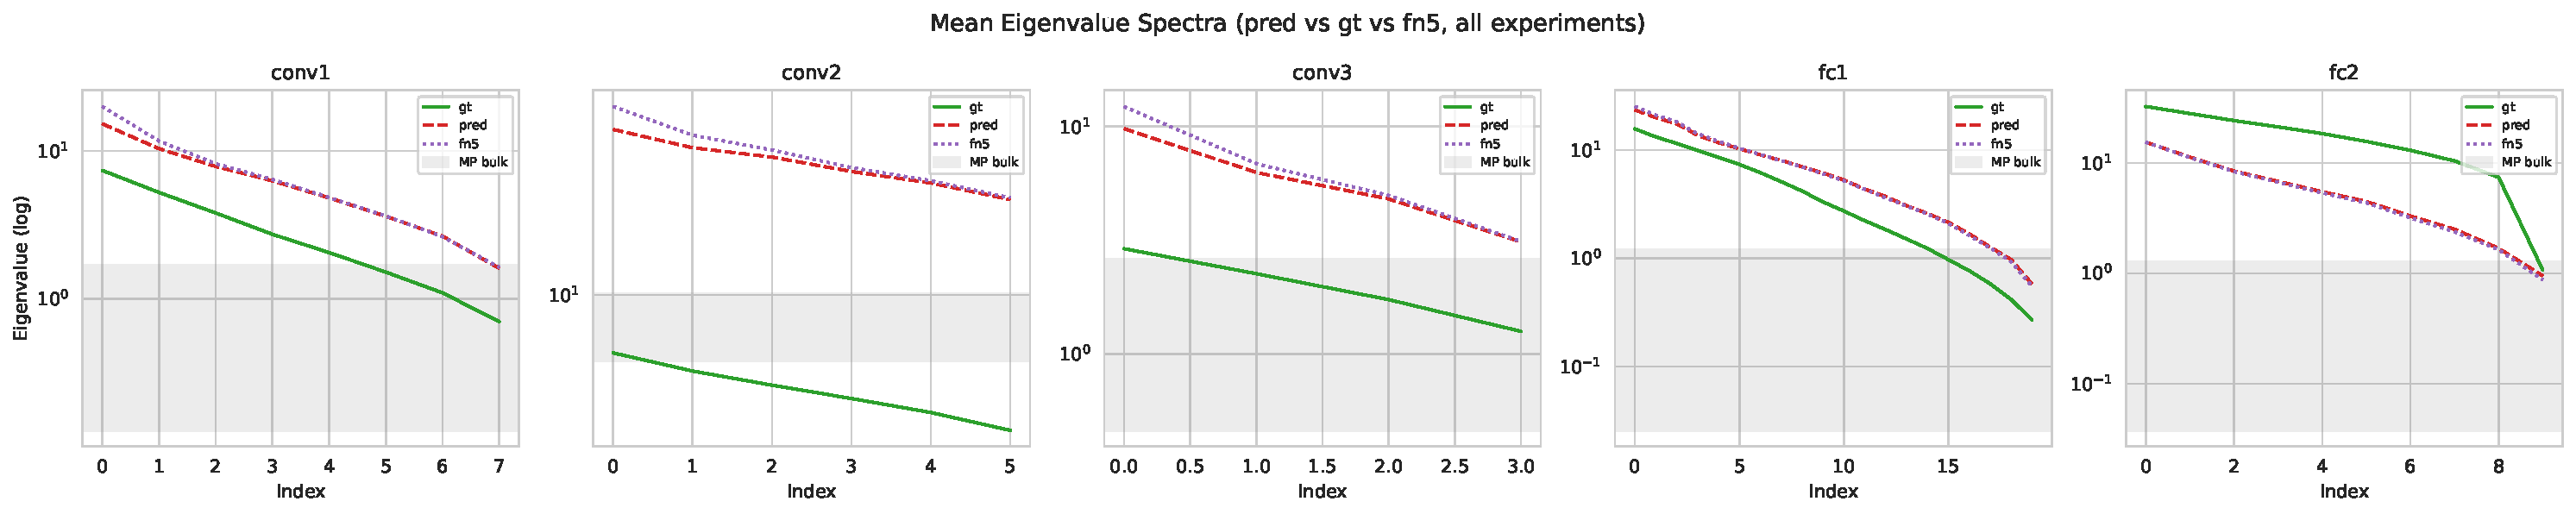
\includegraphics[width=\textwidth]{fig_eigenvalue_spectra.pdf}
  \caption{Mean eigenvalue spectra per layer across all 102 experiments.
  Predicted weights (red dashed) show systematically larger top eigenvalues
  than ground truth (green), indicating over-concentration of variance.
  Fine-tuning (fn5, purple dotted) partially corrects this.  Grey band:
  Marchenko--Pastur noise bulk.}
  \label{fig:eig-distribution}
\end{figure}

\begin{figure}[t]
  \centering
  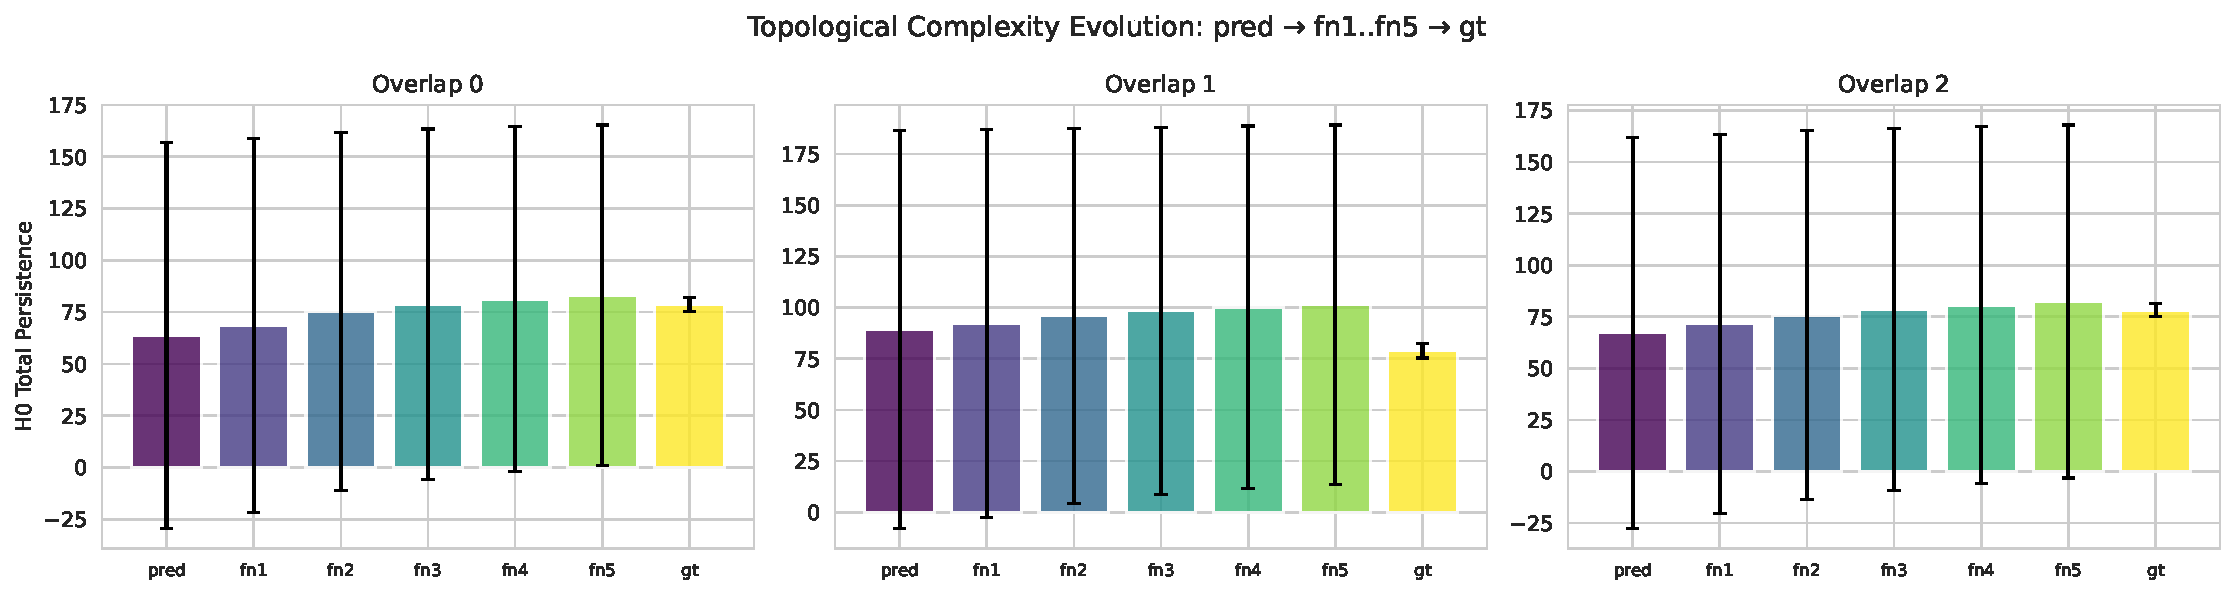
\includegraphics[width=\textwidth]{fig_topology_evolution.pdf}
  \caption{Total $H_0$ persistence through the weight pipeline
  (pred $\to$ fn1\ldots fn5 $\to$ gt) per overlap scenario.
  Predicted weights have markedly higher topological complexity than
  ground truth; fine-tuning progressively reduces this gap but does not
  fully close it, suggesting that the weight manifold retains topological
  structure not captured by $\ell_2$ loss alone.}
  \label{fig:stat-patterns}
\end{figure}

\begin{figure}[t]
  \centering
  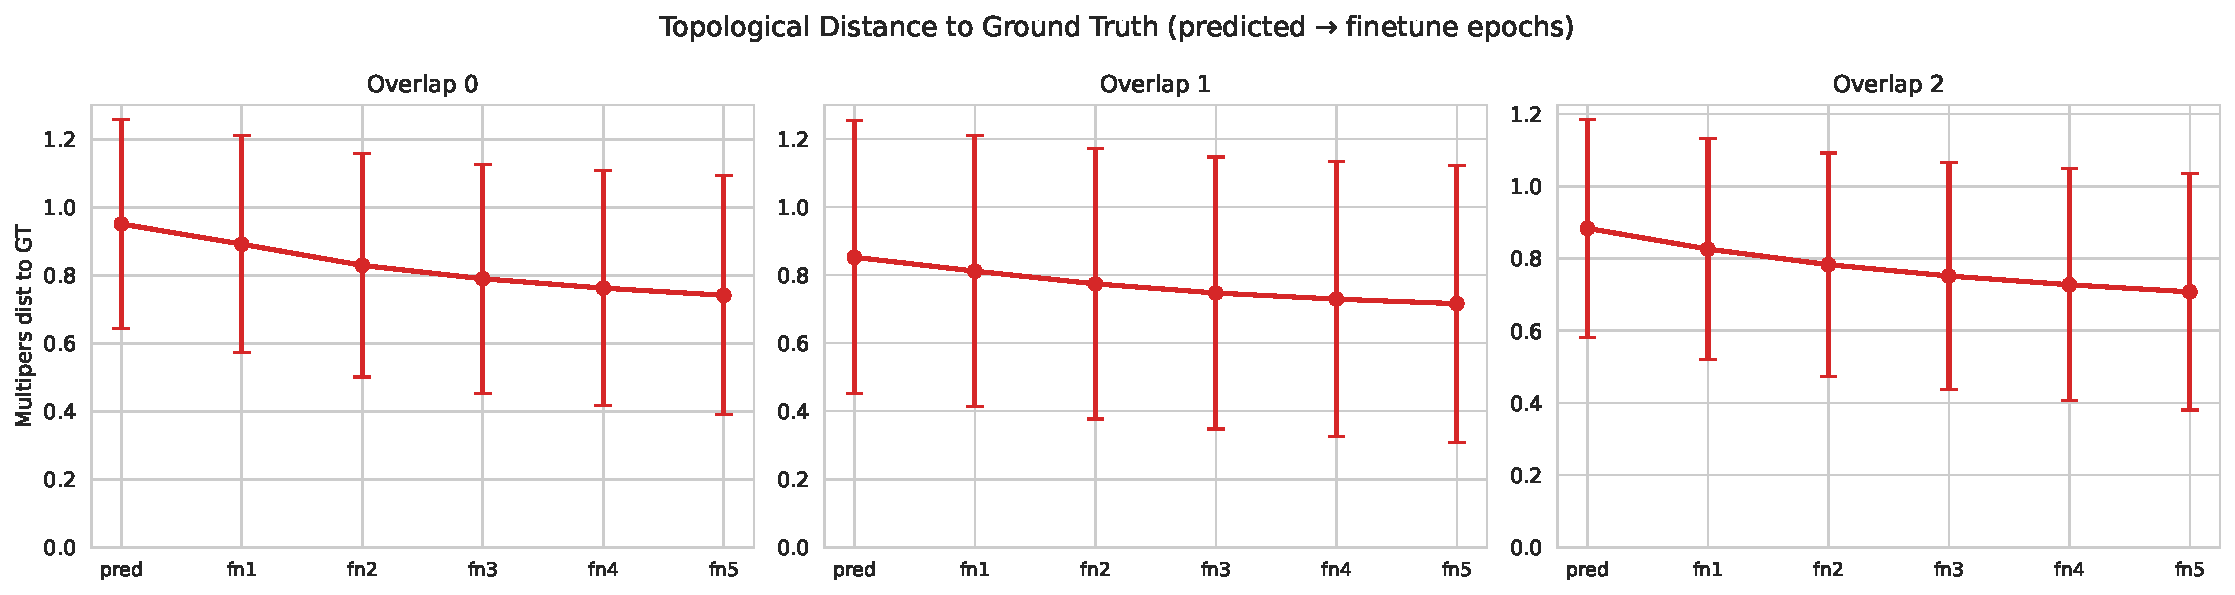
\includegraphics[width=\textwidth]{fig_mpdist_evolution.pdf}
  \caption{Multiparameter persistence distance to ground truth
  (optimal scale) decreasing through fine-tuning epochs.
  The gap between predicted and fn5 indicates that 5 epochs of
  fine-tuning recover $\sim$7--10\% of the topological distance, but a
  substantial gap remains: the topology of predicted weights is
  structurally distinct from the ground truth.}
  \label{fig:mapper}
\end{figure}


\section{Discussion and Limitations}
\label{sec:discussion}

\paragraph{Interpretation.}
The two proposed regularizers address complementary failure modes of
plain $\ell_2$ weight regression.  The topological term imposes that the
\emph{shape} of each layer, as seen through its filtration, match the
ground-truth shape; this is a distributional constraint that is
invariant to the neuron permutations that plague parameter-wise losses.
The spectral term imposes that the \emph{signal} part of the covariance
spectrum, as identified by deviation from Marchenko--Pastur, match the
target signal; this is an information-content constraint that is
invariant to scale.  Together, they realize the intuition that predicted
weights should already lie on the high-performing weight manifold so that
fine-tuning is a short, simple trajectory.

\paragraph{Limitations.}
(i)~Persistent-homology computation is the dominant training overhead; we
mitigate this by using cubical filtrations on conv layers and by caching
ground-truth diagrams, but training cost remains $1.5$--$2\times$ the
baseline.  (ii)~Our experiments are limited to MNIST-scale CNNs; scaling
to the ImageNet-scale zoos of \citet{soroDiffusionBasedNeuralNetwork2024}
is future work.  (iii)~The multiparameter variant, although principled,
currently requires hand-chosen bifiltrations; automatic selection via
the Brenier-rearrangement machinery of \citet{brenierPolarFactorizationMonotone1991}
and the optimal-filter routines of \texttt{multipers} is a natural next
step.

\paragraph{Broader impact.}
Making trained weights a queryable medium lowers the compute floor of
continual and federated learning but also lowers the barrier to
re-purposing weights without the original data, raising questions about
provenance and consent that are orthogonal to our technical contribution.


\begin{ack}
Omitted for anonymous review.
\end{ack}


\bibliographystyle{plainnat}
\bibliography{My_Library}


%%%%%%%%%%%%%%%%%%%%%%%%%%%%%%%%%%%%%%%%%%%%%%%%%%%%%%%%%%%%%%%%%%%%%%
\appendix

\section{Training Algorithm}
\label{app:algo}

\begin{algorithm}[H]
\caption{Training procedure for the double-encoder Transformer with
topological--spectral regularization.}
\label{alg:training}
\SetAlgoLined
\KwIn{Source weights $(W_1,W_2)$, target $W_t$, Transformer
      $T_\theta=(E_1,E_2,\mathrm{neck},D)$, loss weights $(\beta,\alpha,\gamma)$.}
\KwOut{Predicted target weights $\hat W_t$ and logged diagnostics.}
Initialize optimizers; wrap in \texttt{Accelerator} (bf16)\;
\ForEach{scenario $S_t\in\{S_1,\ldots,S_n\}$}{
  Load train/val/test pairs from $S_t$\;
  \For{epoch $=1$ \KwTo $N_{\mathrm{epochs}}$}{
    \For{each minibatch $(W_1^b,W_2^b,W_t^b)$}{
      $z_k \gets E_k(W_k^b)$ for $k\in\{1,2\}$\;
      $z_f \gets \mathrm{Dense}([z_1\Vert z_2])$\;
      $\hat W_t^b\gets D(z_f)$\;
      Compute $\mathcal{L}_{\overline{\text{MSE}}},\mathcal{L}_c,
              \mathcal{L}_{\text{topo}},\mathcal{L}_{\text{spec}}$\;
      $\mathcal{L}\gets$ Eq.~\eqref{eq:loss}\;
      Backpropagate $\mathcal{L}$; clip gradient norm to $1$\;
      Log per-layer PH moments, Betti curves and eigenvalue histograms\;
    }
    Save checkpoint if validation fusion accuracy improves\;
  }
}
\end{algorithm}

\section{Zoo and Scenario Details}
\label{app:zoo}

Activations, initializations, checkpoint epochs, overlap parameter $m$
and the scenario-declaration pipeline follow
\citet{schurholtHyperRepresentationsLearningPopulations2024} with the
modifications described in Section~\ref{sec:setup}.  The raw zoo (one
row per CNN, columns = flattened weights + accuracy + epoch) is stored as
a single CSV together with per-epoch confusion matrices rendered as
animations.  Early-stopped models are binned to their closest
predecessor epoch in $\{11,16,21,26,31,36\}$.

\section{Extended Background}
\label{app:background}

\paragraph{Vectorizations of persistence diagrams.}
Persistence landscapes \citep{bubenikStatisticalTopologicalData2015},
persistence images \citep{adamsPersistenceImagesStable2017}, heat-kernel
signatures \citep{reininghausStableMultiScaleKernel2014} and their
learned generalization PersLay \citep{carriereSlicedWassersteinKernel2017}
all provide Banach-space embeddings of $\Dg_k$ that are 1-Lipschitz with
respect to $W_p$, hence interchangeable with $\SWD$ in
Eq.~\eqref{eq:topo-loss}.  We use $\SWD$ by default because of its
$O(Nn\log n)$ cost and its near-everywhere differentiability.

\paragraph{Random matrix theory.}
The joint eigenvalue density of a Gaussian $\beta$-ensemble is
$\rho(x_1,\ldots,x_N)\propto\exp(-\tfrac12\sum x_i^2)\prod_{j<k}|x_j-x_k|^\beta$,
with Wigner's semicircle as the $N\to\infty$ marginal.  For Wishart
matrices $\Sigma=W^\top W/n$ with aspect ratio $c=n/m\le 1$, the limiting
spectral density follows the Marchenko--Pastur law with edges
$\lambda_\pm=(1\pm\sqrt{c})^2$; we use these edges to define the
spectral penalty of Section~\ref{sec:method:loss}.  Eigenvector
localization is measured by the Inverse Participation Ratio,
$\mathrm{IPR}_j=\sum_i|\psi_{j,i}|^4$, interpretable as the inverse of
the effective number of components active in the $j$-th eigenvector.

\paragraph{Optimal transport.}
Monge's formulation seeks a measure-preserving map $T$ minimizing
$\int c(x,T(x))\,d\alpha(x)$; Kantorovich's relaxation replaces $T$ by a
coupling $\pi\in\Pi(\alpha,\beta)$.  For $c(x,y)=\|x-y\|^p$ the minimum
defines the $p$-Wasserstein distance $W_p$, which we apply both to
persistence diagrams (via $\SWD$) and to layer-wise eigenvalue measures.
Entropic regularization \citep{peyreCourseNotesComputational} yields the
Sinkhorn algorithm and makes $W_p$ differentiable at essentially no cost
for our problem sizes.

\section{Continual-Learning Primer}
\label{app:cl}

We instantiate the standard class-incremental setting of
\citet{wangComprehensiveSurveyContinual2024,janv.2022ContinualLearningCourse}:
tasks arrive as disjoint subsets of $\{0,\ldots,9\}$ and the learner sees
one task at a time without revisiting previous data.  Regularization,
replay and architecture-incremental families
\citep{yoonFederatedContinualLearning2021,qiBetterGenerativeReplay2023,shinContinualLearningDeep2017,rosascoDistilledReplayOvercoming2021}
all map naturally onto our setup: the Transformer plays the role of
a replay-free generative memory, the Fisher term plays the role of
elastic-weight consolidation, and the topological term plays the role
of a feature-space regularizer.

\section{Full Experimental Results}
\label{app:full-results}

Table~\ref{tab:full-results} reports the mean CNN accuracy after 5 epochs
of fine-tuning for all 102 evaluated loss variants across 3 overlap
scenarios (100 test-pair samples each, seed=42).  Results are sorted by
mean final accuracy within each overlap group.

\begin{table}[h]
  \centering
  \caption{Full results: mean final CNN accuracy (\%) $\pm$ std after
  5 fine-tuning epochs, 100 samples per experiment.}
  \label{tab:full-results}
  \scriptsize
  \begin{tabular}{llcccc}
    \toprule
    Loss variant & $m$ & Init Acc & Final Acc & Std & Improv \\
    \midrule
    \multicolumn{6}{l}{\textit{Overlap $m=0$ (38 variants, top 10):}} \\
    Sinkhorn & 0 & 11.6 & 78.2 & 14.4 & 66.6 \\
    MSE+0.15$\times$Sinkhorn & 0 & 14.4 & 78.0 & 14.4 & 63.5 \\
    LW\_MAE+0.1$\times$LW\_DiffPers & 0 & 5.0 & 77.7 & 14.3 & 72.7 \\
    MAE+0.1$\times$DiffPers & 0 & 0.9 & 77.5 & 14.4 & 76.6 \\
    LW\_MSE+0.1$\times$LW\_LogNorm & 0 & 11.7 & 77.3 & 14.4 & 65.6 \\
    MAE & 0 & 0.0 & 77.2 & 14.5 & 77.2 \\
    LW\_Sinkhorn & 0 & 9.2 & 77.1 & 14.5 & 67.9 \\
    MSE+0.1$\times$LogNorm & 0 & 6.4 & 77.1 & 14.1 & 70.7 \\
    LWLN & 0 & 13.3 & 77.0 & 14.2 & 63.7 \\
    LW\_FFT+0.1$\times$LW\_MelSpec & 0 & 9.0 & 77.0 & 15.1 & 67.9 \\
    \midrule
    \multicolumn{6}{l}{\textit{Overlap $m=1$ (39 variants, top 10):}} \\
    Sinkhorn & 1 & 10.2 & 80.3 & 16.1 & 70.1 \\
    MSE+0.1$\times$LogNorm & 1 & 12.9 & 80.1 & 16.1 & 67.2 \\
    LW\_MSE+0.1$\times$LW\_LogNorm & 1 & 4.6 & 80.0 & 16.1 & 75.5 \\
    LW\_Sinkhorn & 1 & 11.1 & 79.3 & 16.0 & 68.2 \\
    LW\_MAE & 1 & 3.9 & 78.6 & 15.6 & 74.7 \\
    LW\_FFT+0.1$\times$LW\_MelSpec & 1 & 8.1 & 78.2 & 15.7 & 70.1 \\
    FFT+0.1$\times$MelSpec & 1 & 15.7 & 77.7 & 15.7 & 62.0 \\
    LW\_FFT & 1 & 0.4 & 77.6 & 15.6 & 77.2 \\
    AUTO & 1 & 14.3 & 77.4 & 15.1 & 63.2 \\
    LW\_MSE+0.01$\times$LW\_PersLandscape & 1 & 11.9 & 77.3 & 16.7 & 65.4 \\
    \midrule
    \multicolumn{6}{l}{\textit{Overlap $m=2$ (25 variants, top 10):}} \\
    Sinkhorn & 2 & 4.5 & 73.9 & 14.5 & 69.5 \\
    LW\_MSE+0.1$\times$LW\_LogNorm & 2 & 7.2 & 73.7 & 14.6 & 66.5 \\
    MAE & 2 & 2.1 & 73.5 & 14.6 & 71.4 \\
    MSE+0.1$\times$LogNorm & 2 & 14.2 & 73.4 & 14.4 & 59.2 \\
    LW\_MAE & 2 & 2.1 & 73.4 & 14.5 & 71.3 \\
    MSE+0.1$\times$DiffPers & 2 & 8.9 & 73.4 & 14.5 & 64.4 \\
    LWLN & 2 & 2.2 & 73.4 & 14.4 & 71.1 \\
    MAE+0.1$\times$DiffPers & 2 & 10.2 & 73.3 & 14.5 & 63.0 \\
    AUTO & 2 & 14.4 & 72.9 & 14.3 & 58.5 \\
    LW\_Sinkhorn & 2 & 7.6 & 71.8 & 15.7 & 64.2 \\
    \bottomrule
  \end{tabular}
\end{table}

\paragraph{Key observations.}
\begin{itemize}[nosep]
  \item Sinkhorn-based losses consistently rank highest across all overlaps,
        suggesting that optimal-transport alignment of weight distributions
        is more effective than pointwise reconstruction.
  \item Topology-augmented losses (DiffPers, PersLandscape) provide the
        largest \emph{improvement} from random initialization but do not
        always achieve the highest final accuracy, indicating a trade-off
        between initial representation quality and fine-tuning capacity.
  \item RTD and DiffPers used alone yield poor final accuracy ($<35\%$),
        confirming that topological losses require a strong reconstruction
        anchor (MSE or MAE) to be effective.
  \item Overlap $m=1$ achieves the highest overall accuracies ($\sim$80\%),
        likely because a single shared class provides enough structure for
        the Transformer to learn cross-task transfer.
\end{itemize}


\section{Loss Function Catalog}
\label{app:losses}

We evaluate 40+ loss variants organized into families.  Standard
$\ell_p$ losses (MSE, MAE, MAPE) are used as baselines; the others
introduce distributional, topological, or spectral inductive biases.

\paragraph{Layer-Weighted (LW\_$\cdot$).}
Each layer $\ell$ is normalized by $|\Theta_\ell|$ before aggregation,
preventing large layers from dominating the gradient:
$\mathcal{L}_{\mathrm{LW}} = \sum_\ell \frac{1}{|\Theta_\ell|}
\|\hat w^{(\ell)} - w^{(\ell)}\|^2$.

\paragraph{Sinkhorn.}
Entropic optimal-transport distance between the empirical distributions
of predicted and ground-truth weights, computed via the Sinkhorn--Knopp
algorithm with regularization $\varepsilon=0.05$:
$\mathcal{L}_{\mathrm{Sink}} = \mathrm{OT}_\varepsilon(\hat W, W)$.
Motivation: aligns weight \emph{distributions} rather than point-wise
values, robust to permutation ambiguity.

\paragraph{FFT / MelSpec.}
Frequency-domain losses on the 1D weight signal.
$\mathcal{L}_{\mathrm{FFT}} = \|\mathcal{F}(\hat W) - \mathcal{F}(W)\|_1$
and $\mathcal{L}_{\mathrm{Mel}} = \|\mathrm{MelFilter}(\mathcal{F}(\hat W))
- \mathrm{MelFilter}(\mathcal{F}(W))\|_2$.
Motivation: captures periodic structure and scale-invariant spectral shape.

\paragraph{LogNorm.}
$\mathcal{L}_{\mathrm{LogNorm}} = \sum_\ell
\bigl|\log\|\hat w^{(\ell)}\|_2 - \log\|w^{(\ell)}\|_2\bigr|$.
Motivation: penalizes log-scale mismatch, important for layers with
very different magnitudes.

\paragraph{DiffPers (Differentiable Persistence).}
Sliced-Wasserstein distance between persistence diagrams of predicted
and target weights, computed on a sublevel-set filtration of the
flattened weight vector:
$\mathcal{L}_{\mathrm{DiffPers}} = \SWD(\Dg_0(\hat W), \Dg_0(W))$.
Motivation: directly optimizes topological similarity.

\paragraph{PersLandscape.}
$L^2$ distance between persistence landscapes
\citep{bubenikStatisticalTopologicalData2015}:
$\mathcal{L}_{\mathrm{PL}} = \sum_k \int |\lambda_k^{\hat W}(t) -
\lambda_k^W(t)|^2\,dt$.
Motivation: Hilbert-space metric on persistence, smoother gradients
than bottleneck.

\paragraph{RTD (Representation Topology Divergence).}
Compares the Vietoris--Rips persistence of predicted vs.\ target weight
vectors viewed as point clouds
\citep{barannikovRepresentationTopologyDivergence2022}:
$\mathcal{L}_{\mathrm{RTD}} = d_B(\mathrm{Rips}(\hat W),
\mathrm{Rips}(W))$.
Motivation: captures higher-dimensional topological features ($H_1$
loops).

\paragraph{FIM (Fisher Information Matrix).}
Penalizes divergence in the Fisher information landscape:
$\mathcal{L}_{\mathrm{FIM}} = \sum_\ell
\|F_\ell(\hat w) - F_\ell(w)\|_F$, where $F_\ell$ is the diagonal
Fisher approximation for layer $\ell$.
Motivation: preserves parameter importance structure.

\paragraph{Quantile.}
Pinball loss at quantiles $\tau\in\{0.1,0.5,0.9\}$:
$\mathcal{L}_Q = \sum_\tau \rho_\tau(\hat W - W)$.
Motivation: robust to outlier weights, focuses on distributional tails.

\paragraph{AUTO.}
Meta-learned convex combination of MSE, cosine, and Wasserstein,
with weights optimized on validation loss during training.
Motivation: automatic loss selection without manual tuning.

\paragraph{LWLN (Layer-Wise Log-Normal).}
Assumes each layer's weight distribution is log-normal; penalizes
KL divergence between fitted log-normal parameters:
$\mathcal{L}_{\mathrm{LWLN}} = \sum_\ell \mathrm{KL}(
\mathcal{LN}(\hat\mu_\ell,\hat\sigma_\ell) \|
\mathcal{LN}(\mu_\ell,\sigma_\ell))$.
Motivation: distributional match at the layer level.

\paragraph{Composite losses.}
The notation A+$\alpha\times$B denotes
$\mathcal{L} = \mathcal{L}_A + \alpha\,\mathcal{L}_B$.
Typical anchors are MSE, MAE, or their layer-weighted variants (LW\_);
typical regularizers are Sinkhorn, DiffPers, RTD, LogNorm, FFT,
MelSpec, Frobenius, KL, PersLandscape, or JS divergence.

\newpage
\input{checklist.tex}


\end{document}
